% !TeX root = ../../ZF_bmicha_Ana.tex
\subsection{Cosinus und Sinus - Integrale \texorpdfstring{\hfill S.74}{S.74}}
    
    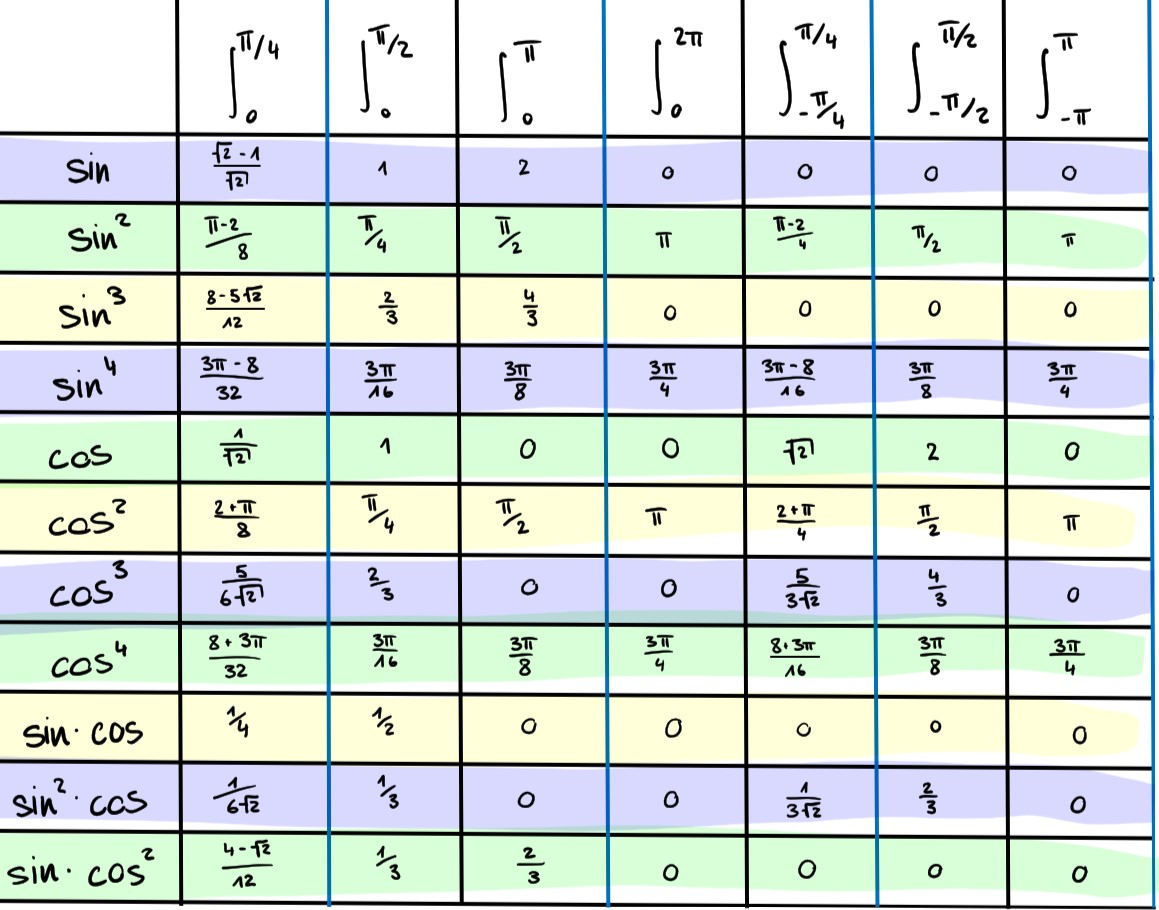
\includegraphics[width = \linewidth]{src/Appendix/integraltabelle_sin_cos.jpg}
    Für $a,b \in \mathbb{N}$ und $n \geq 2$, gelten:
    \begin{align*}
        \int_{a \cdot \frac{\pi}{2}}^{b \cdot \frac{\pi}{2}} \sin^n(x) \ dx 
            &= \frac{n-1}{n} \int_{a \cdot \frac{\pi}{2}}^{b \cdot \frac{\pi}{2}} \sin^{n-2}(x) \ dx\\[0.5em]
        \int_{a \cdot \frac{\pi}{2}}^{b \cdot \frac{\pi}{2}} \cos^n(x) \ dx 
            &= \frac{n-1}{n} \int_{a \cdot \frac{\pi}{2}}^{b \cdot \frac{\pi}{2}} \cos^{n-2}(x) \ dx
    \end{align*}